\documentclass[10pt]{beamer}
\usepackage{amsmath}
\usepackage{amssymb}
\usepackage{geometry}
\usepackage{graphicx}
\usepackage{url}
\usepackage{bm}

\makeatletter
\let \@sverbatim \@verbatim
\def \@verbatim {\@sverbatim \verbatimplus}
{\catcode`'=13 \gdef \verbatimplus{\catcode`'=13 \chardef '=13 }} 
\makeatother

\begin{document}

\begin{frame}
\large
Lecture 6:\\
Dummy Variable Regression\\
STAT 632, Spring 2020
\end{frame}

\begin{frame}
\begin{itemize}
\item So far we have only considered explanatory variables that are quantitative such as a person's height, or the diameter of a tree.
\vspace{5pt}
\item An \textbf{indicator} or \textbf{dummy} variable is an explanatory variable that only takes on two possible numeric values (e.g., 0 or 1). 
\vspace{5pt}
\item In simple linear regression, dummy variables allow us to compare the means of two groups.  The concept can be further generalized in multiple linear regression to problems involving more than two groups. 
\end{itemize}
\end{frame}

\begin{frame}{Example}
\begin{itemize}
\item Data set from Ebay for the game Mario Kart for the Nintendo Wii.
\vspace{5pt}
\item Consider a simple linear regression model relating the total price to the dummy variable for game condition (new or used).
\end{itemize}
\begin{align*}
x_i = \begin{cases}
  1, & \text{if $i^{th}$ game is new}\\
  0, & \text{if $i^{th}$ game is used}
\end{cases}
\end{align*}

\begin{align*}
Y_i = \beta_0 + \beta_1 x_i + e_i 
= \begin{cases}
\beta_0 + \beta_1 + e_i, & \text{if $i^{th}$ game is new}\\
\beta_0 + e_i, & \text{if $i^{th}$ game is used}
\end{cases}
\end{align*}
\end{frame}

\begin{frame}[fragile]
\small
\begin{verbatim}
> library(openintro)

# remove outliers
> ind <- which(marioKart$totalPr > 100)
> marioKart2 <- marioKart[-ind, ]

# create dummy variable
> n <- nrow(marioKart2)
> marioKart2$cond01 <- rep(0, n)
> marioKart2$cond01[marioKart2$cond == 'new'] <- 1
\end{verbatim}
\end{frame}

\begin{frame}[fragile]
\small
\begin{verbatim}
> lm1 <- lm(totalPr ~ cond01, data = marioKart2)
> summary(lm1)

Coefficients:
            Estimate Std. Error t value Pr(>|t|)    
(Intercept)   42.871      0.814  52.668  < 2e-16 ***
cond01        10.900      1.258   8.662 1.06e-14 ***
---
Signif. codes:  0 ‘***’ 0.001 ‘**’ 0.01 ‘*’ 0.05 ‘.’ 0.1 ‘ ’ 1

Residual standard error: 7.371 on 139 degrees of freedom
Multiple R-squared:  0.3506,	Adjusted R-squared:  0.3459 
F-statistic: 75.03 on 1 and 139 DF,  p-value: 1.056e-14
\end{verbatim}
\end{frame}

\begin{frame}[fragile]
\small
\begin{verbatim}
> plot(totalPr ~ cond01, data = marioKart2, xaxt='n', 
       xlim=c(-0.1, 1.1), xlab = 'Condition', ylab = 'Total Price')
> axis(1, at=c(0,1), labels=c('Used (0)', 'New (1)'))
> abline(lm1)
\end{verbatim}

\begin{figure}
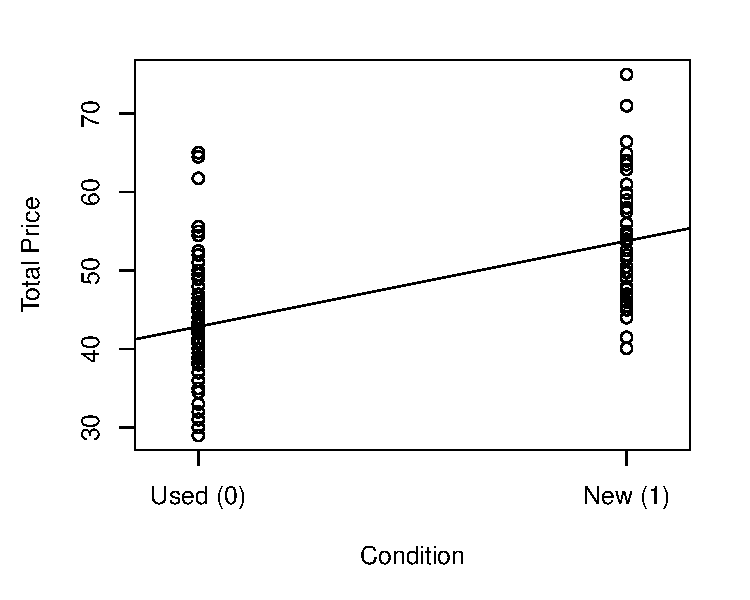
\includegraphics[scale=0.5]{figure/price_cond.pdf}
\end{figure}
\end{frame}

\begin{frame}{Interpretation}
Equation for the least squares regression line from R summary:\\
$$\hat{y} = 42.87 + 10.9 x$$

\begin{itemize}
\item The intercept $\hat{\beta}_0 = 42.87$ is the estimated average price when the game is in used condition (x = 0).
\vspace{5pt}
\item $\hat{\beta}_0 + \hat{\beta}_1 = 42.87 + 10.9 = 53.77$ is the estimated average price when the game is in new condition (x=1).
\vspace{5pt}
\item The slope $\hat{\beta}_1 = 10.9$ indicates that, on average, a new game sells for \$10.9 dollars more than a used game.
\end{itemize}
\end{frame}

\begin{frame}[fragile]{}
We can also interpret a confidence interval for the slope $\beta_1$.

\begin{verbatim}
> confint(lm1)
                2.5 %   97.5 %
(Intercept) 41.261713 44.48048
cond01       8.411621 13.38754
\end{verbatim}
\vspace{10pt}

We are 95\% confident that the average price of a new game is between \$8.41 and \$13.39 more than a used game.
\end{frame}

\end{document}